\chapter{Réseaux programmables avec SDN}

On cherche à concevoir une architecture plus adaptée aux enjeux de la communication actuelle discutés dans le chapitre 1. Cette problématique a amené scientifiques et les ingénieurs impliqués à concevoir \gls{sdn}. \gls{sdn} est un nouveau \glslink{paradigme}{paradigme} réseau qu'on est actuellement en cours de développer pour adapter l'infrastructure existante à ce nouveau scénario.
Le but de ce chapitre est de (re)définir SDN et de présenter en quoi SDN répond aux besoins explicités dans le chapitre 1.
%Ce chapitre répond aux questions : Qu'est-ce que SDN ? Qu'est-ce que cela propose ?


\section{Séparation de l'intelligence (contrôle) de la commutation (flux de données)}

%Having recognized the problem, the networking commu- nity is hard at work developing programmable networks, such as GENI [1] a proposed nationwide research facility for experimenting with new network architectures and dis- tributed systems. These programmable networks call for programmable switches and routers that (using virtualiza- tion) can process packets for multiple isolated experimen- tal networks simultaneously.
Ayant adressé cette problématique, la communauté réseau fait beaucoup d'efforts pour le développement des réseaux programmables. Ces réseaux utilisent des switches et des routeurs programmables qui peuvent traiter des paquets pour des multiples réseaux expérimentaux  à la fois, grâce à la \gls{virtualisation}. \cite{OpenFlowStanfordOssification} Divers projets pour les réseaux programmables, comme NETCONF \cite{NETCONF}, Ethane \cite{Ethane}, GENI \cite{GENI} etc. ont été réalisés et en ont servi de base pour ce paradigme qu'on développe et supporte aujourd'hui : SDN. 

%SDN is described in this article with the Open Networking Foundation (ONF) [1] definition: “In the SDN architecture, the control and data planes are decoupled, network intelli- gence and state are logically centralized, and the underlying network infrastructure is abstracted from the applications.”

SDN est défini au long de cette étude  selon \gls{onf} : Dans l'architecture SDN, les plans de contrôle et de données sont découpés, l'intelligence et l'état du réseau sont logiquement centralisés, et l'infrastructure du réseau est donc abstraite des applications. \cite{SDNNewNormONFExecutiveSummary}


%The control plane is responsible for configuration of the node and programming the paths that will be used for data flows. Once these paths have been determined they are pushed down to the data plane. Data forwarding at the hardware level is based on this control information.

Le \gls{controlplane} est responsable pour la configuration d'un nœud et pour la programmation des chemins qui seront utilisés par les flux de données. Le \gls{dataplane} fourni au hardware les informations nécessaires à la commutation. \cite{ImplementationChallengesForSDNBackground}



Dans l'architecture réseau traditionnellement déployée, chaque équipement actif contient un plan de contrôle et un plan de données à l'intérieur du même matériel. L'ossification d'internet discuté dans le chapitre 1 est largement attribuée à ce fort couplage entre les deux plans provocant que toutes les décisions sur les flux de donnés soient embarquées dans chaque élément réseau. La manque d'une interface de contrôle commune à tous les dispositifs complique toute évolution que cela soit un simple changement de configuration ou le développement d'une nouvelle application. \cite{SurveySDNArchi}



%As mentioned previously, the so-called Internet “ossifica- tion” [2] is largely attributed to the tight coupling between the data– and control planes which means that decisions about data flowing through the network are made on-board each network element. In this type of environment, the deployment of new network applications or functionality is decidedly non- trivial, as they would need to be implemented directly into the infrastructure. Even straightforward tasks such as config- uration or policy enforcement may require a good amount of effort due to the lack of a common control interface to the various network devices.

Avec SDN, on propose la séparation de ces deux éléments. Le \gls{controlplane} est implémenté par un contrôleur centralisé et commun à tous les équipements qui passent à contenir seulement le \gls{dataplane} en plus d'un module de communication.  La séparation de la fonction de commutation de la logique de contrôle permet un déploiement plus facile de nouveaux protocoles et applications. La virtualisation et le management du réseau deviennent plus simples et les nombreux \glspl{middlebox} sont consolidés dans le logiciel de contrôle. \cite{SurveySDNArchi} \cite{SDNNewNormONFExecutiveSummary}
%the separation of the forwarding hardware from the control logic allows easier deployment of new protocols and applications, straightforward network visualization and management, and consolidation of various middleboxes into software control.

Dans l'image ci-dessous on voit un schéma illustrant l'ensemble de l'architecture dans les deux cas.

%\begin{figure}[!h] %on ouvre l'environnement figure
%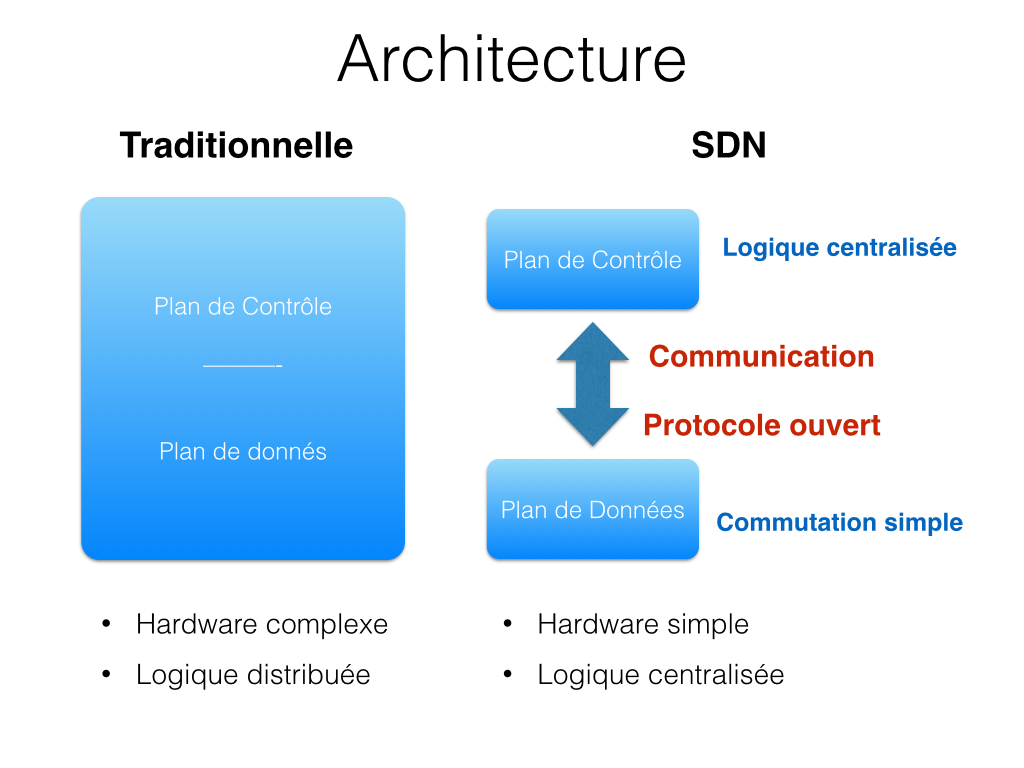
\includegraphics[width=15cm]{images/ComparaisonArchis.png} %ou image.png, .jpeg etc.
%\caption{ Un équipement actif dans l'Architecture Traditionnelle et SDN} %la légende
%\label{imgNodesArchi} %l'étiquette pour faire référence à cette image
%\end{figure} %on ferme l'environnement figure



\begin{figure}[!h] %on ouvre l'environnement figure
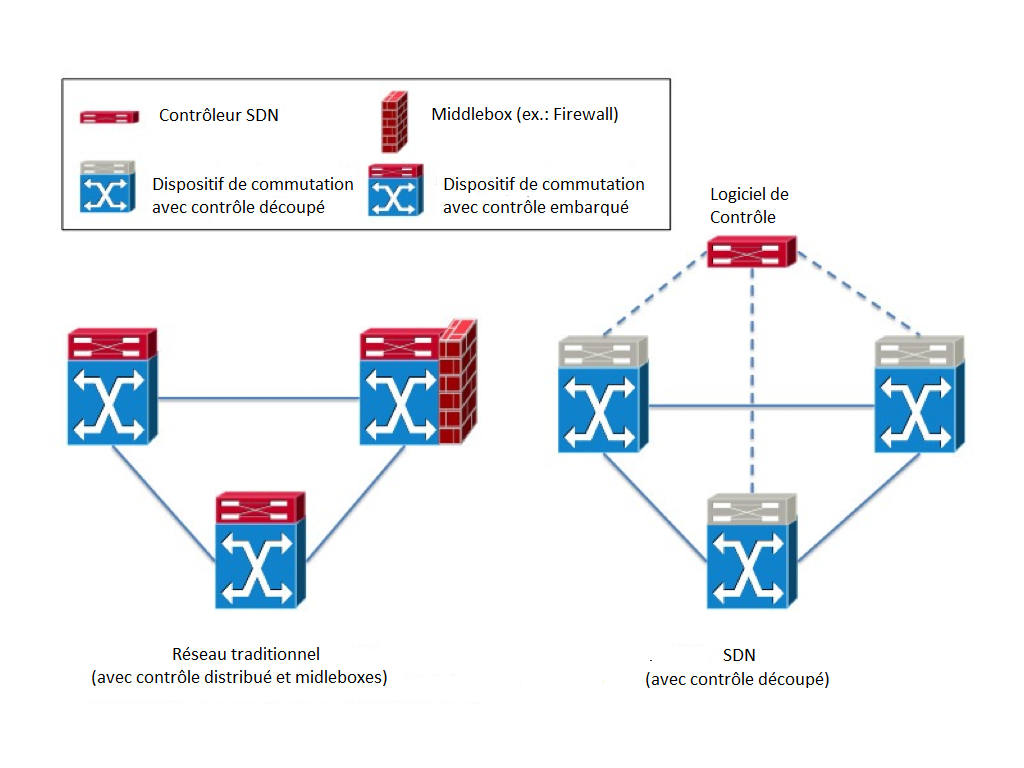
\includegraphics[width=15cm]{images/TraditionalVsSDN.png} %ou image.png, .jpeg etc.
\caption{ L'ensemble de l'Architecture Traditionnelle et SDN \cite{SurveySDNArchi}} %la légende
\label{imgOverviewArchi} %l'étiquette pour faire référence à cette image
\end{figure} %on ferme l'environnement figure


Comme on voit dans l'image, traditionnellement chaque dispositif actif de l'infrastructure contient un \gls{controlplane} et un \gls{dataplane} embarqués. Dans cette architecture le contrôle est dit distribué et implique la décision de commutation réalisée dans chaque nœud. Cette approche est aussi appelée, réseau dirigé par configuration où le comportement du réseau dépend de la configuration de chaque équipement actif.  \gls{ip} et \gls{mpls} sont exemples de ce modèle avec le contrôle distribué. Ces systèmes comptent avec l'échange de routes et d'informations de joignabilité qui résultent en \glspl{dataplane} programmés pour réaliser ces chemins. La haute disponibilité est fourni grâce à la redondance, avec l'approche "deux de tous" où on duplique chaque nœud permettant des chemins alternatifs lors de la faille d'un lien ou d'un élément. \cite{sdnbookControlDataPlanes}


Dans le cas de SDN, le contrôle est centralisé et chaque dispositif réalise seulement la fonction de commutation. L'avantage sortant de ce modèle est la possibilité d'avoir une vue du réseau permettant de simplifier la programmation du contrôle. SDN n'est pas la seule solution de contrôle centralisé et de réseau programmable existante. Indépendamment, dans tous les cas, cette approche permet aux applications de ne plus prendre conscience de l'état de chaque nœud, mais d'interagir avec un contrôle unique s'en occupant de ces détails. \cite{sdnbookControlDataPlanes}

%This allows a simpler and more flexible network control and management, and also network virtualization.
%SDN technologies enable us to address the high- bandwidth, dynamic nature of computer networks; adapt the net- work functions to different business needs easily; and reduce network operations and management complexity significantly. sndChineseBookConceptsApplications


%From these service-focussed requirements, SDN has emerged. Control is moved out of the individual network nodes and into the separate, centralized controller. SDN switches are con- trolled by a Network Operating System (NOS) that collects information using the API shown in Figure 2B and manipulates their forwarding plane, providing an abstract model of the network topology to the SDN controller hosting the applications.

\section{Contrôle centralisé et hardware simplifié : l'intérêt de SDN}

%SDN profite du fait que la majorité des switches et routeurs existants contiennent des tableaux de flux qui exécutent à une fréquence ligne pour implémenter leurs protocoles et collecter des statistiques. \cite{OpenFlowStanfordSwitch} 


Cette séparation permet de simplifier et rendre plus flexible le contrôle et le management du réseau. Les technologies SDN adaptent plus facilement les fonctions du réseau aux besoins de différents business tout en réduisant significativement la complexité des opérations et du management, et par conséquent les coûts opérationnels. \cite{sndChineseBookConceptsApplications}


La séparation des plans de contrôle et de données leur permet d'évoluer indépendamment. Les éléments de commutation deviennent plus stables ayant un plus petit et moins volatile code de base. 
Le principal avantage d'un contrôle centralisé est la vue du réseau qu'il peut fournir et la simplification de la programmation du contrôle.

Avec l'approche \gls{sdn}, les switches sont contrôlés par un \gls{nos} qui fourni un modèle abstrait de la topologie du réseau au contrôleur \gls{sdn} hébergeant les applications. Le contrôleur peut donc exploiter cette vue globale du réseau pour optimiser le management des flux et supporter les requis de 'scalabilité' et de flexibilité. \cite{WhySDN}

Avec le \gls{controlplane} et le \gls{dataplane} embarqués, les éléments actifs échangent leurs paramètres à travers de protocoles de routage (comme RIP, BGP, OSPF etc.) avec les voisins pour acquérir des informations pertinentes sur le réseau et prendre les décisions de commutation des paquets entrants. Dans ce modèle les changements d'états du réseau sont transférés entre les voisins et le temps pour qu'ils deviennent cohérents est appelé temps de convergence. Ce système implique l'utilisation de complexes algorithmes de calcul de route qui doivent s'exécuter dans chaque nœud à chaque changement d'état et doit aussi traiter la problématique d'un bouclage de diffusion entre les voisins. Avec SDN, la prise de décision est centralisée, ce qui évite la gestion de ces échanges et l'exécution multiple de ces algorithmes qui est faite qu'une fois dans le contrôleur. \cite{sdnbookControlDataPlanes}


%SDN technology can also help with the challenge of nebulous network perimeters. Vague boundaries make it impossible to determine where to deploy security devices such as firewalls. SDN technology can help by allowing administrators to route all (internal and perimeter) traffic through one central firewall. And there’s an additional benefit of network traffic flowing through a single point: It facilitates real-time capture and analysis of IDS and IPS data.

La technologie SDN peut aussi aider avec le challenge des périmètres réseaux floues. Les vagues frontières empêchent de déterminer où placer les dispositifs de sécurité, tels que firewall. SDN permet le routage de tout trafic à travers un firewall centralisé. Un avantage en plus d'avoir un trafic réseau qui passe par un point unique est de faciliter la capture et l'analyse en temps réel des données \gls{ids} et \gls{ips}. \cite{sdnbookControlDataPlanes}

\section{Choix d'implémentation pour des challenges}

%Cette partie présente quels sont les enjeux pour déployer SDN, ayant pour but d'identifier les challenges lors de sa mise en place. Pour chaque enjeux, les approches pour les surmonter sont montrées tout en proposant les compromis de ces propositions.

Le premier point à noter pour l'implémentation de SDN impose les notions de contrôle logiquement centralisé et de contrôle physiquement centralisé. Alors que la centralisation du contrôle est considérée comme un élément clé de la technologie, sa centralisation physique pose des sur la 'scalabilité' et la disponibilité. Un contrôle physiquement devient un point unique de failles pour tout le réseau et impose son remplacement lors d'une évolution. De cette manière, une topologie où le contrôle est logiquement centralisé mais physiquement distribué semble être plus logique. \cite{sdnbookControlDataPlanes}



Un des objectifs de SDN est de développer des réseaux construits sur du matériel d'usage général. Avec une interface programmable sur du matériel standard, un réseau équipé avec des multiples fournisseurs devient une possibilité. Cependant, cette flexibilité impose un challenge quant à la performance. Avec un processeur d'usage général, les langages de programmation haut-niveau et divers outils de design fournissent une abstraction qui permet le développement rapide de sophistiquées fonctions de traitement de paquets. En contrepartie, des processeurs avec architecture optimisée pour le traitement réseau peuvent atteindre une performance plus élevée mais la flexibilité d'implémentation est réduite. Encore une fois, une architecture hybride semble être plus cohérente, satisfaisant le meilleur compromis entre performance et flexibilité. \cite{ImplementationKeyChallenges}